% Lecture 18, Fig. 1: hypocentre and epicentre of an earthquake on a dipping fault (cross-section).
\documentclass[tikz,border=6pt]{standalone}
\usepackage{mathpazo}
\usetikzlibrary{arrows.meta,shapes.geometric}
\begin{document}
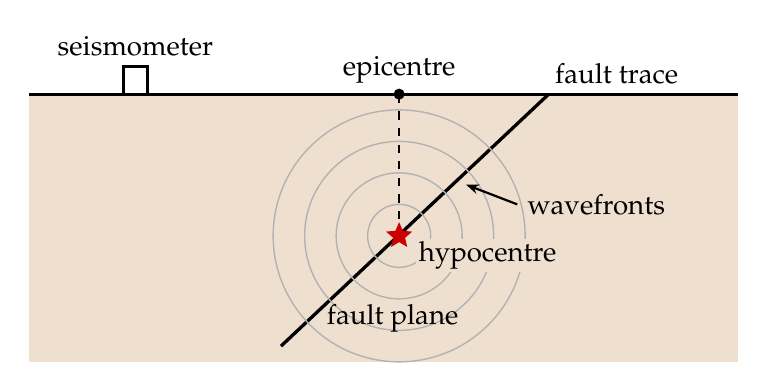
\begin{tikzpicture}[line width=0.8pt]
  \fill[brown!25!white] (0,0) rectangle (9,3.4);
  \draw[line width=1pt] (0,3.4) -- (9,3.4);                       % surface
  \draw[line width=1.2pt] (6.6,3.4) -- (3.2,0.2);                 % fault plane
  \coordinate (H) at (4.7,1.6);
  \coordinate (E) at (4.7,3.4);
  \foreach \r in {0.4,0.8,1.2,1.6} \draw[gray!60, line width=0.5pt] (H) circle (\r);
  \draw[dashed] (H) -- (E);
  \node[star, star points=5, star point ratio=2.2, fill=red!80!black, inner sep=1.6pt] at (H) {};
  \fill (E) circle (2pt);
  \node[right, fill=brown!25!white, inner sep=1pt] at (4.9,1.35) {hypocentre};
  \node[above] at (E) {epicentre};
  \node[above right] at (6.55,3.4) {fault trace};
  \node[right] at (3.65,0.55) {fault plane};
  \draw[-{Stealth[length=1.6mm]}] (6.2,2.0) node[right] {wavefronts} -- (5.55,2.25);
  % seismometer
  \draw[line width=1pt] (1.5,3.4) -- (1.5,3.75) -- (1.2,3.75) -- (1.2,3.4);
  \node[above] at (1.35,3.75) {seismometer};
\end{tikzpicture}
\end{document}
